\section{Coordenogramas}



De acordo com a norma DIS-NORM-036, a corrente transitória de magnetização (\textit{inrush}) e o ponto ANSI podem ser obtidos a partir da corrente nominal do transformador ($I_{nom,trafo} = 500 \; kVA / \sqrt{3} 13.8 \; kV = 21 \; A$). 

A corrente de \textit{inrush} pode ser determinada como 6 vezes a corrente nominal do transformador num tempo de 0.1 segundos:

\begin{center}
$I_{INRUSH} = 6I_{nom,trafo} = 6 \cdot 21 = 126 \; A$ \\ 
\end{center}

O ponto ANSI para a impedância em p.u do transformador de aproximadamente 6\%, num tempo de 4 segundos, resulta em uma corrente:

\begin{center}
$I_{ANSI} = 16.6I_{nom,trafo} = 16.6 \cdot 21 = 348.6 \; A$ \\ 
\end{center}

Definidos esses pontos, os coordenogramas de fase e neutro podem ser traçados de acordo com as figuras \ref{fig:fase} e \ref{fig:neutro}.

\begin{figure}[H] 
    \centering
    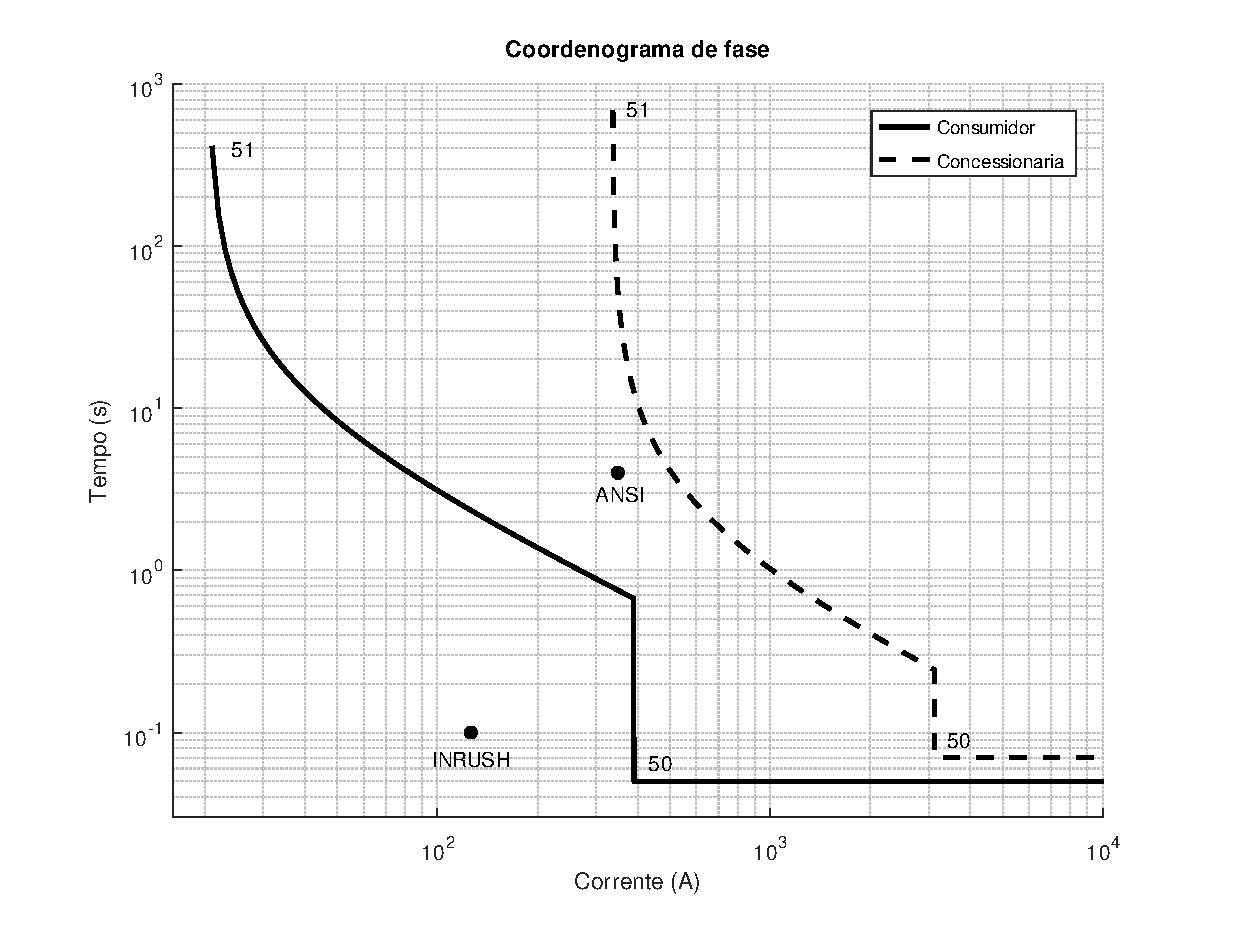
\includegraphics[width=0.9\textwidth]{images/fase.eps}
    \caption{Coordenograma de fase. A curva da unidade 51 do relé da concessionária é do tipo 0.15-MI-IEC, enquanto que para o consumidor é do tipo 0.9-MI-IEC.}
    \label{fig:fase}
\end{figure}

\begin{figure}[H] 
    \centering
    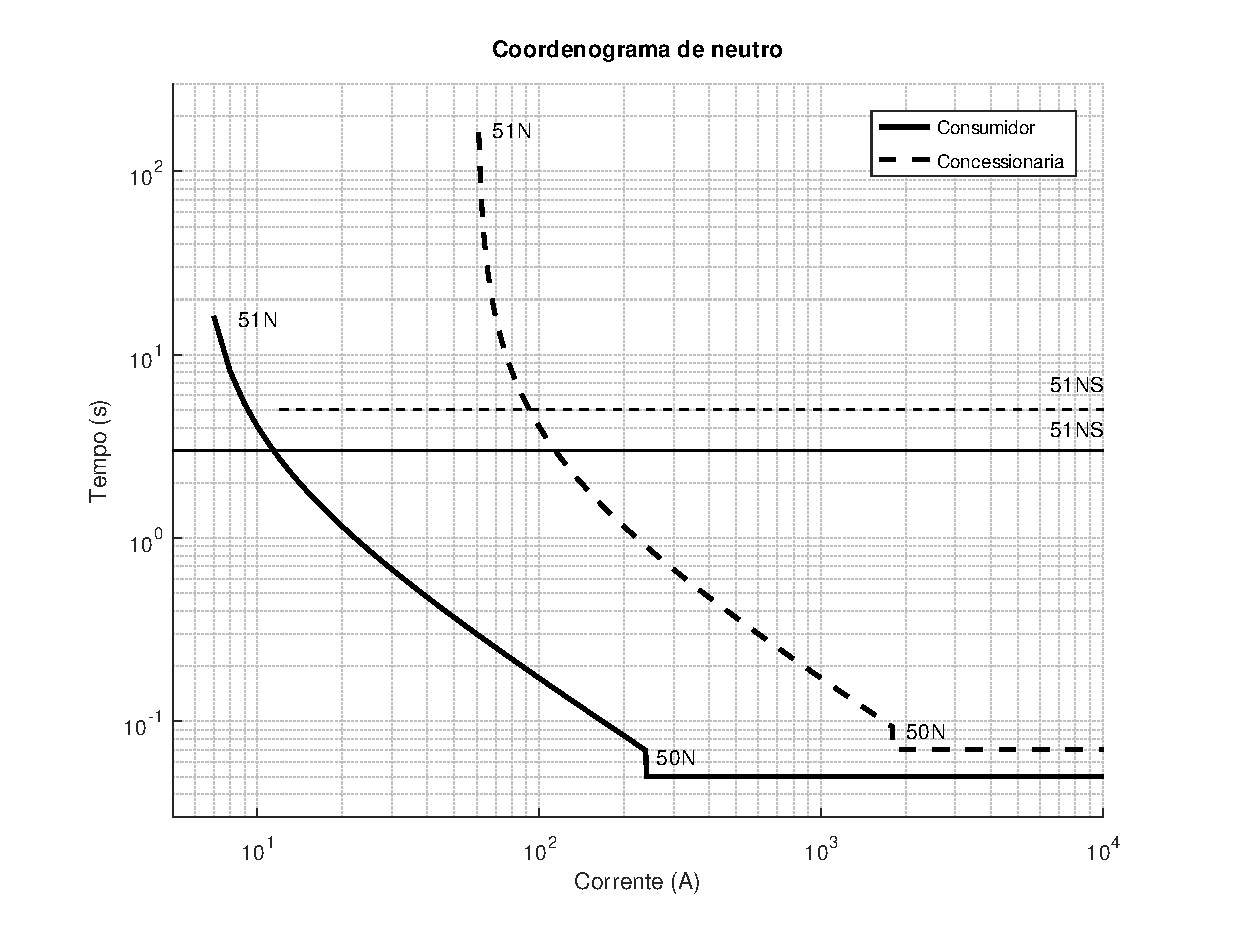
\includegraphics[width=0.9\textwidth]{images/neutro.eps}
    \caption{Coordenograma de neutro. A curva da unidade 51N do relé da concessionária e do consumidor são ambas do tipo 0.2-MI-IEC.}
    \label{fig:neutro}
\end{figure}

Conforme observado nos coordenogramas, as curvas determinadas para as unidades 51/51N/51NS/50/50N do relé URPE 7104T garantem uma operação coordenada com as correspondentes unidades do relé do alimentador da concessionária.
